\begin{frame}
	\frametitle{Klimamodelle - Überblick}
	\begin{columns}
	\column{0.65\linewidth}
	\begin{figure}
		\centering
		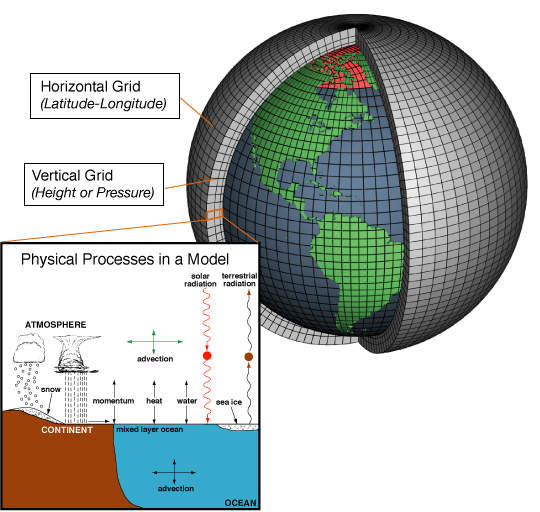
\includegraphics[width=0.8\linewidth]{%
				bilder/AtmosphericModelSchematic.png}
		\caption{Schematische Abbildung eines Klimamodells, Quelle: NOAA}
	\end{figure}
	\column{0.35\linewidth}
	\begin{itemize}
		\item Klimamodelle bestehen aus Differentialgleichungen
		\item Es gelten Erhaltungssätze (Energie, Impuls, Masse)
		\item Ströhmungslehre und Chemie werden berücksichtigt.
		\item Berechnet werden unter anderem Wind, Wärmetransfer, Strahlung, Luftfeuchtigkeit und Oberflächenhydrologie
	\end{itemize}
	\end{columns}

	\note{
		\begin{itemize}
			\item[] Klimamodelle sind Computersimulationen, die Differentialgleichungen (Navier-Stokes) nutzen um die chemischen und physikalischen Prozesse des Erdklimas nachzubilden.
			\item[] Das erste Klimamodell enthielt Atmosphäre, Ozean, Landmassen und Seeeis, deckte aber nur \nicefrac{1}{6} der Erdoberfläche ab (Nordpol bis Äquator über einen Winkel von \SI{120}{\degree}).
			\item[] 1956 erstes Modell, dass saisonale Wettermuster reproduzieren konnte.
			\item[$\rightarrow$] general circulation models werden entwickelt.
			\item[$\rightarrow$] Weiterentwicklungen sind Atmospheric (AGCMs) und oceanic GCMs (OGCMs), sowie atmosphere-ocean coupled general circulation models (CGCM or AOGCM).
			\item[] Standard Auflösung eines OGCM (HadOM3): \SI{1.25}{\degree} in Längen- und Breitengrad, mit 20 vertikalen Leveln $\rightarrow$ etwa 1,5 mio. Variablen.
		\end{itemize}
		Typische Parameter eines atmosphärischen Zirkulationsmodells:
		\begin{itemize}
			\item[] Luftdruck, Konvektion, Oberflächenprozesse
			\item[] Albedo, Hydrologie, Wolkenbedeckung
    	\item[] horizontale Geschwindigkeitskomponenten der Atmosphärenschichten
    	\item[] Temperatur und Wasserdampf der Atmosphärenschichten
    	\item[] Solare (Sonne) und Infratotstrahlung (Reflexion der Erde)
		\end{itemize}
	}
\end{frame}

\begin{frame}
	\frametitle{Klimamodelle - im IPCC}
	\begin{figure}
		\begin{columns}
			\column{0.65\linewidth}
				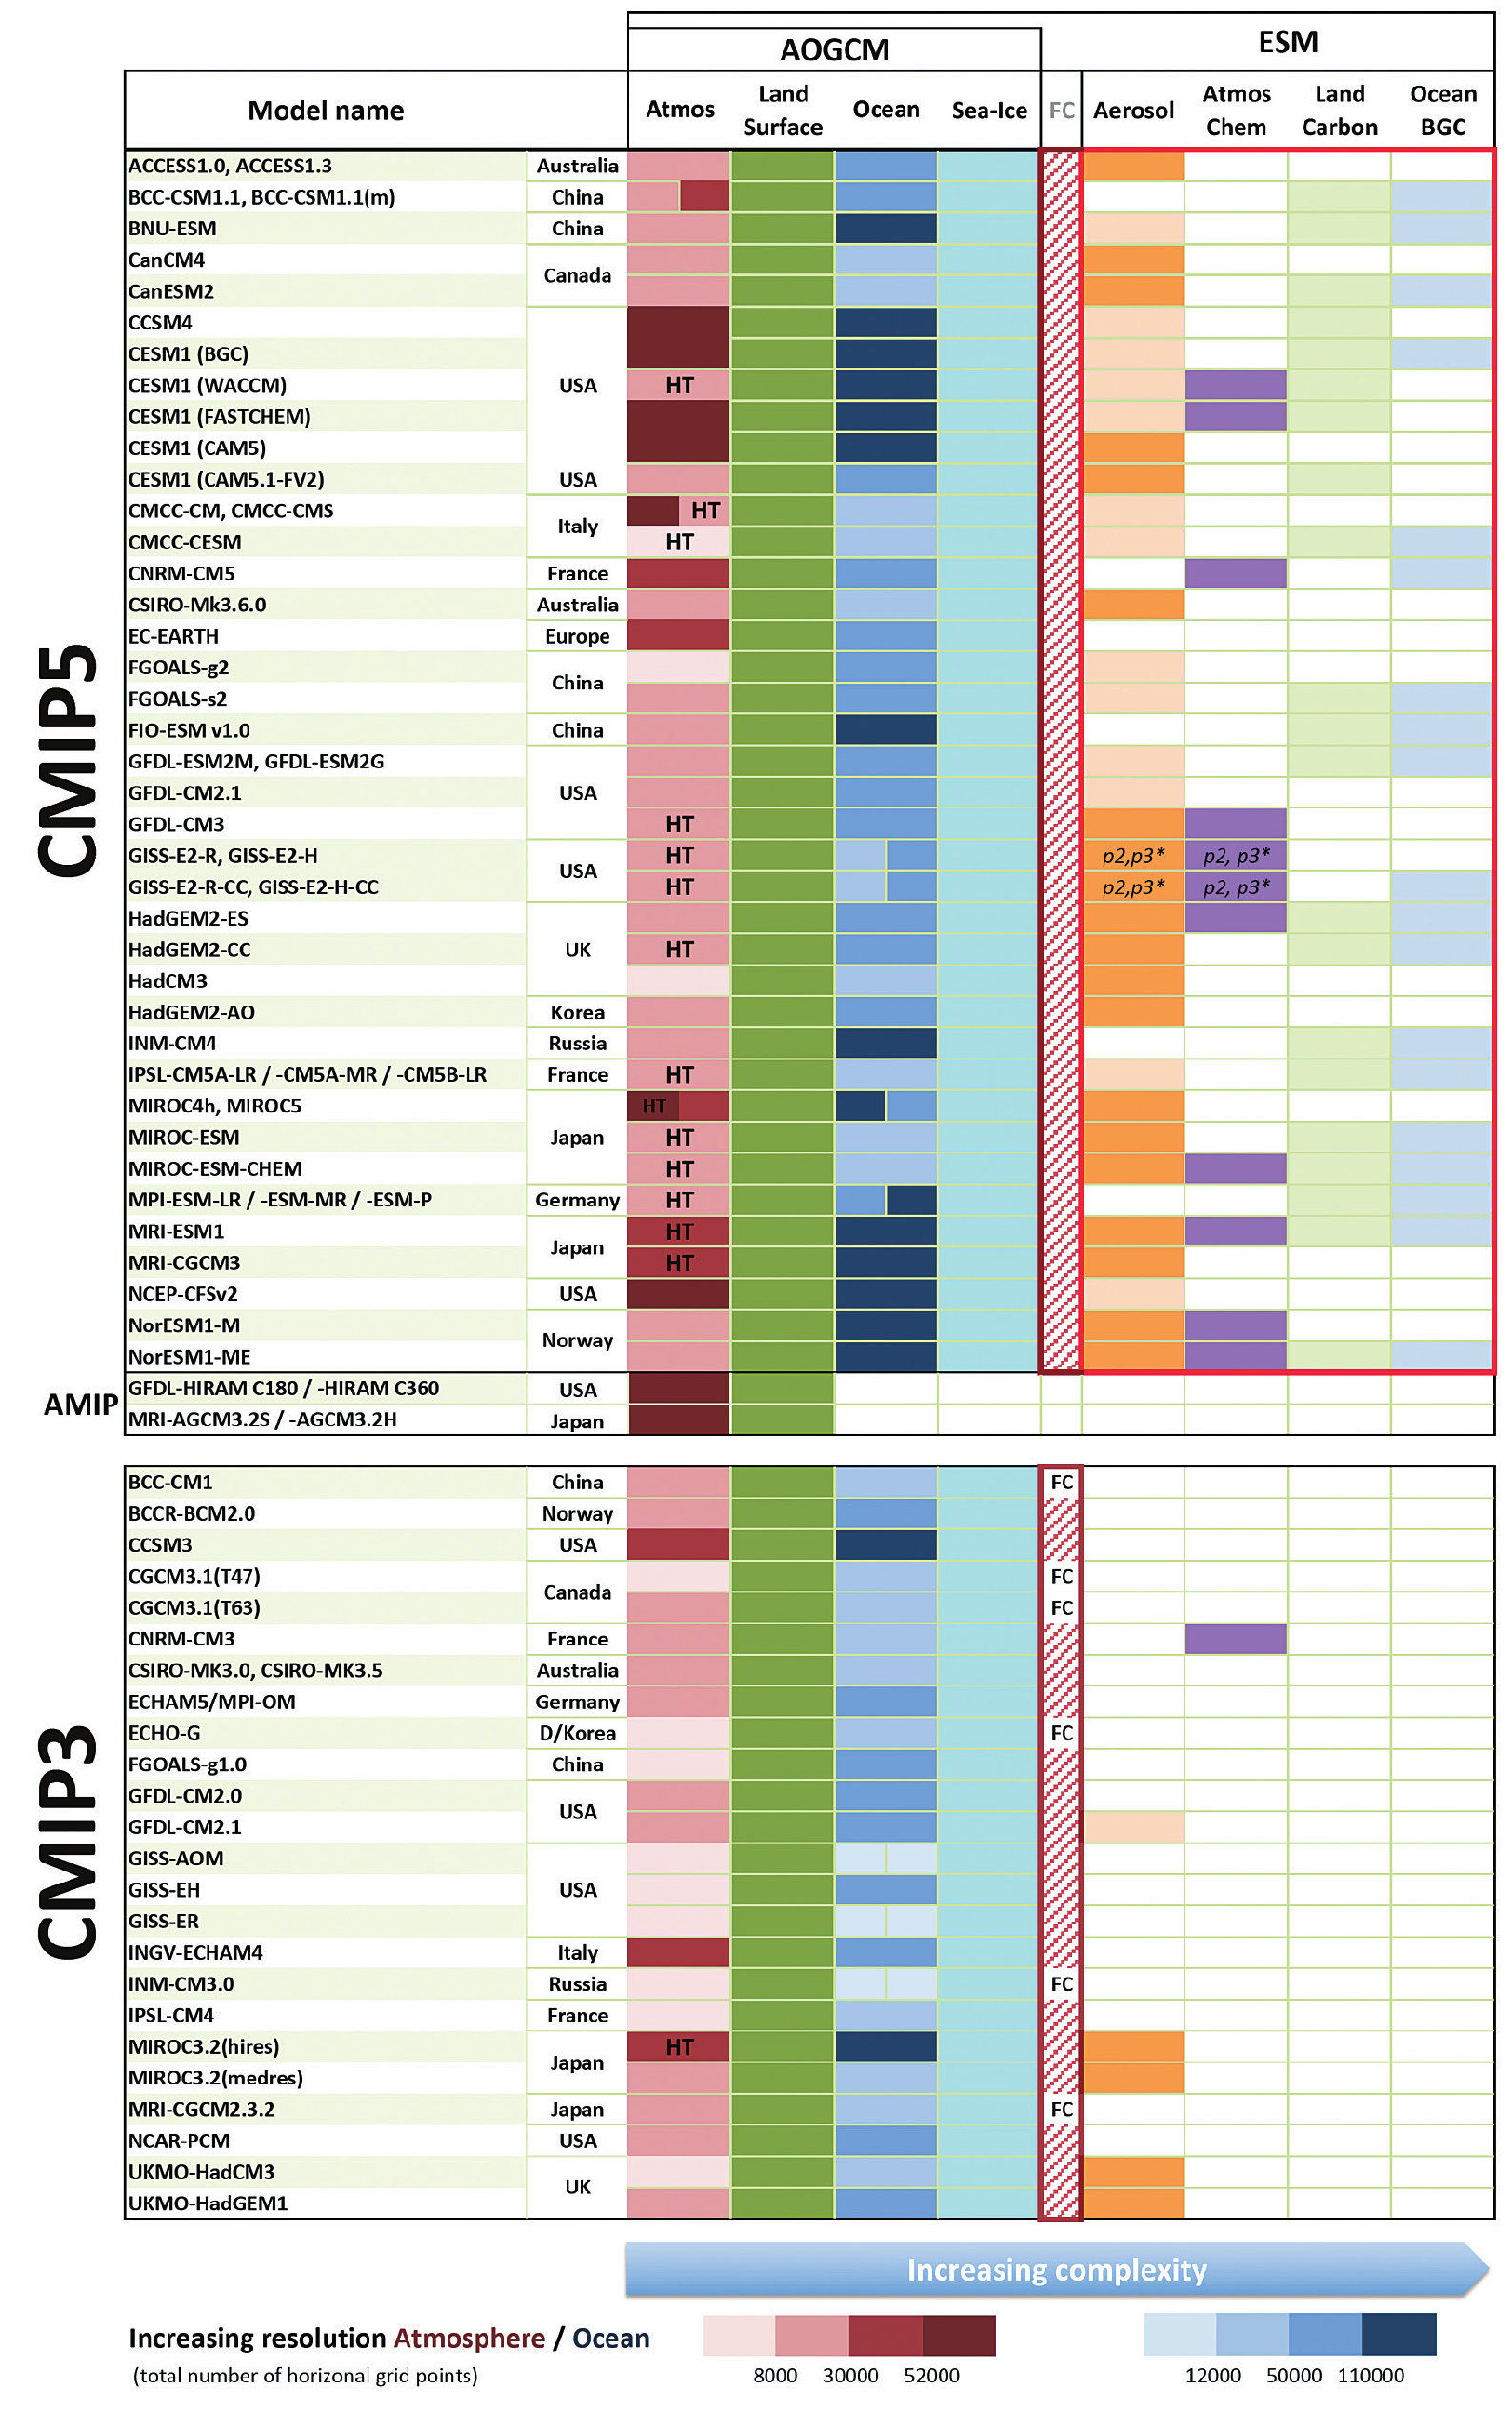
\includegraphics[trim={0cm 8.5cm 0cm 0cm}, clip,width=0.95\linewidth]{bilder/klimamodelle_ipcc_2013.png}
			\column{0.35\linewidth}
				\caption{Verwendete Klimamodelle im IPCC, Quelle: IPCC 2013 Kapitel 9}
		\end{columns}
	\end{figure}

	\note{
	\begin{itemize}
		\item[CMIP5] Coupled Model Intercomparison Project Phase 5
		\item[$\rightarrow$] von CIMP3 nach CIMP5 erhöhte Komplexität und Auflösung, sowie mehr Modelle
		\item[AOGCM] Atmosphere–Ocean General Circulation Models
		\item[ESM] Earth System Models
		\item[HT] High-Top Atmosphäre, mit kompletter Stratosphäre und einem Model über der Stratopause
		\item[AMIP] Nur Atmosphäre und Landmassen
		\item[] Genaue Details zu den Modellen im IPCC 2013 Kapitel 9
		\item[] Farbgebung, falls physikalische Gleichung mit wenigstens zwei-wege Kopplung an andere Komponente (erlaubt Klimafeedbacks).
		\item[] Die Auflösung an Land ist typischerweise vergleichbar mit der Auflösung der Atmosphäre.
		\item[] Die Auflösung des Seeeises ist üblicherweise vergleichbar mit der Auflösung des Ozeans.
	\end{itemize}
	}
\end{frame}
